\documentclass[border=2mm]{standalone}
\usepackage{tikz}

% define normal distribution function 'normaltwo'
\def\normaltwo{\x,{4*1/exp(((\x-3)^2)/2)}}
% input y parameter
\def\y{4.4}
% this line calculates f(y)
\def\fy{4*1/exp(((\y-3)^2)/2)}

\begin{document}
	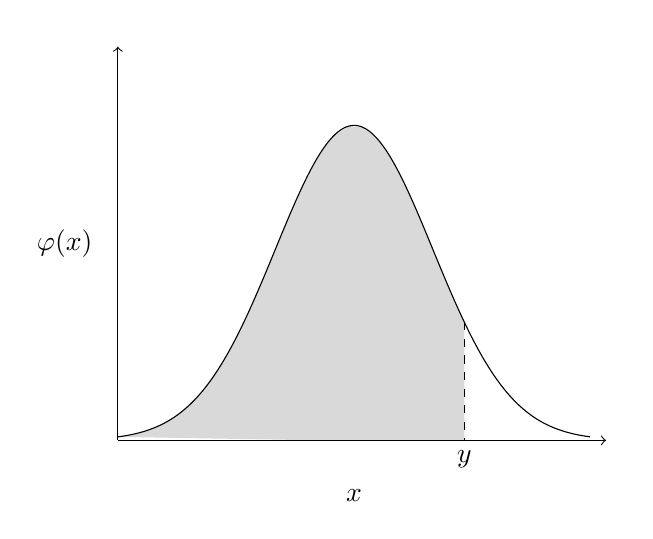
\begin{tikzpicture}
		% Shade gray area underneath curve.
		\fill [fill=gray!30] (2.6,0) -- plot[domain=0:4.4] (\normaltwo) -- ({\y},0) -- cycle;
		% Draw and label normal distribution function
		\draw[color=black,domain=0:6] plot[samples=1000] (\normaltwo) node[right] {} ;
		%\draw[color=blue,domain=0:6] plot (\normaltwo) node[right] {};
	 
		% Add dashed line dropping down from normal.
		\draw[dashed] ({\y},{\fy}) -- ({\y},0) node[below] {$y$};
	 
		% Optional: Add axis labels
		\draw (-.2,2.5) node[left] {$\varphi(x)$};
		\draw (3,-.5) node[below] {$x$};
	 
		% Optional: Add axes
		\draw[->] (0,0) -- (6.2,0) node[right] {};
		\draw[->] (0,0) -- (0,5) node[above] {};	 
	\end{tikzpicture}
\end{document}
